% !TEX encoding = UTF-8
% !TEX TS-program = pdflatex
% !TEX root = ../tesi.tex
\null\newpage
%**************************************************************
\chapter{Approfondimenti}
%**************************************************************

\section{Funzionamento di Hibernate} 
\label{sec:appendice-1}
Come avviene la conversione delle tabelle in classi Java?\\
\begin{figure}[h]
	\centering
	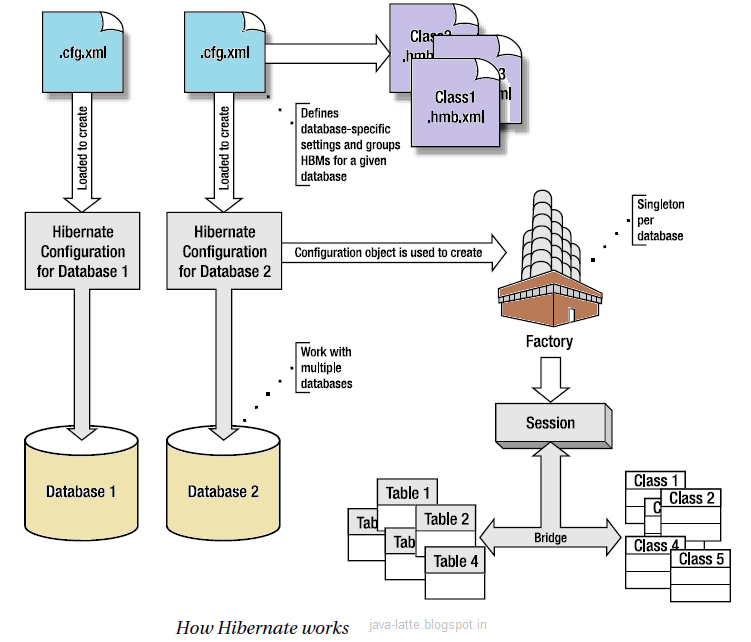
\includegraphics[height = 5 cm]{hibernate_works}
	\caption{Schema del funzionamento di Hibernate}
	\label{schema-generale-hibernate}
\end{figure}
Hibernate deve conoscere la configurazione del database e per farlo necessita di un file, estesi generalmente in \textbf{.cfg.xml}. Al framework è inoltre indispensabile fornire dei files di mapping, uno per ogni tabella e generalmente estesi con i suffissi \textbf{.hmb.xml}, che contengono le informazioni riguardanti le colonne della singola tabella da trasformare in un oggetto Java.\\

\begin{figure}[h]
	\centering
	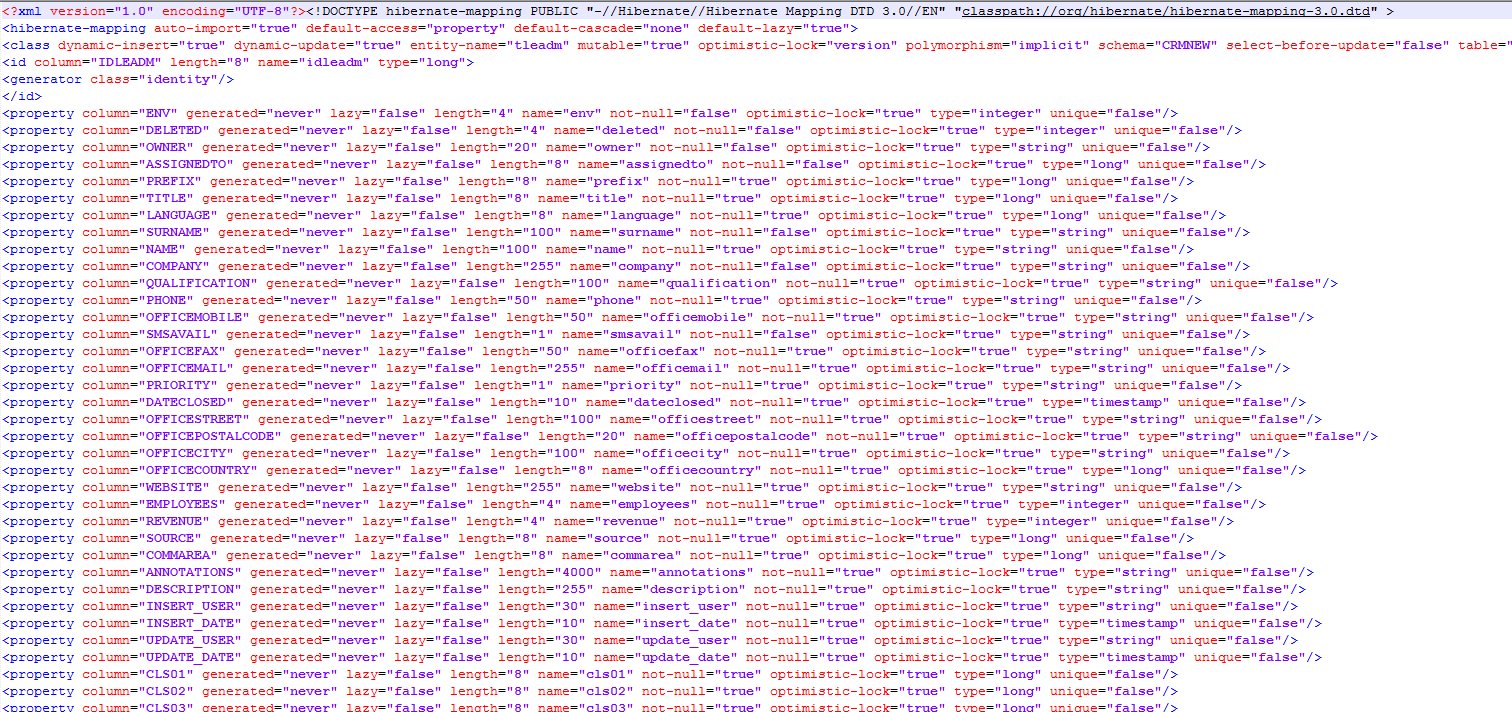
\includegraphics[height = 5 cm]{hibernate-entities}
	\caption{XML di un'entità Hibernate di JGalileo CRM}
	\label{entità}
\end{figure}

Questi files vengono poi utilizzati per creare una \emph{SessionFactory} globale e thread-safe che funge da \emph{gateway} per l'interrogazione del database. \\ I vantaggi dell'utilizzo della tecnica di programmazione ORM (Object-Relational Mapping) sono molteplici ed in particolare consentono:
\begin{itemize}
	\item \textbf{Disaccoppiamento dal DBMS};
	\item \textbf{Elevata portabilità};
	\item \textbf{Drastica riduzione del codice sorgente}, a causa dei semplici comandi che mascherano complesse istruzioni;
	\item \textbf{Elevata modularità}.
\end{itemize}

\section{Model View Controller}
\label{sec:MVC}
Il pattern \emph{MVC, Model-View-Controller}, è un design pattern, cioè uno schema di progettazione che costituisce una soluzione progettuale ad un problema ricorrente \hyperlink{01}{[1]}.\\
\'E uno dei pattern più famosi ed utilizzati per la separazione tra la logica di presentazione e la logica di business nei sistemi software, ed in particolare nelle applicazioni web.\\
\begin{figure}[h]
	\centering
	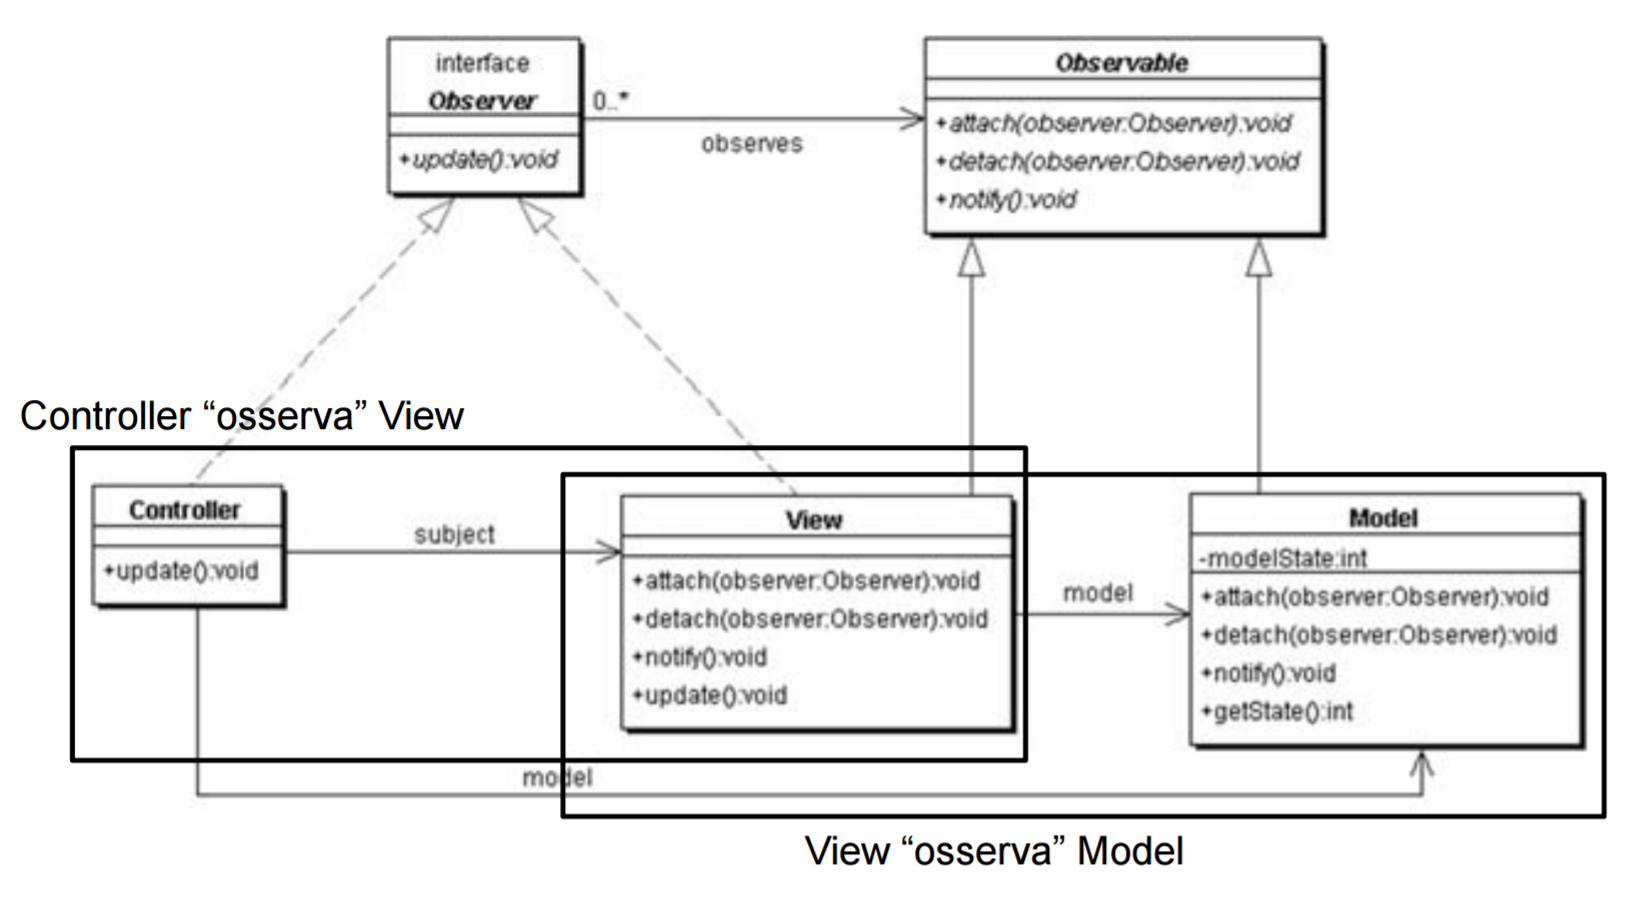
\includegraphics[height = 7 cm]{MVC}
	\caption{Design pattern MVC}
	\label{mvc-schema}
\end{figure}
Come evidenziato dalla figura \ref{mvc-schema}, vi sono 3 attori principali:
\begin{itemize}
	\item \textbf{Model}: rappresenta la cosiddetta \emph{logica di business}, cioè l'insieme di dati e metodi per eseguire operazioni;
	\item \textbf{View}rappresenta come i dati vengono visualizzati nell'interfaccia utente, cioè la \emph{logica di presentazione};
	\item \textbf{Controller}:si pone come intermediario tra view e model;
\end{itemize}
Il controller, che osserva la view, riceve da quest'ultima le richieste di elaborazione e, una volta che il model restituisce i dati, si occupa di inviarli alla view.\\
Questo design pattern ha molti lati positivi, tra i quali la divisione dei compiti ed il riuso di codice.\\


\newpage